\documentclass[english,aspectratio=169]{beamer}
% \usepackage{fontspec}
\usepackage{graphicx}
\usepackage{amssymb}
\usepackage{booktabs}
\usepackage{siunitx}

% \setmainfont[Mapping=tex-text]{DejaVu Serif}
% \setsansfont[Mapping=tex-text]{DejaVu Sans}
% \setmonofont{DejaVu Sans Mono}

\newcommand{\fb}{\si{\femto\barn}}
\newcommand{\invfb}{\si{\per\femto\barn}}

\usetheme[]{bjeldbak}

\begin{document}

\title[4t X-Section]{Four Tops Cross Section Measurement}

\subtitle{Trilepton Channel}

\author[C. Fangmeier]{Caleb Fangmeier}

\institute[UNL]{University of Nebraska \-- Lincoln}

\date{\today}

\titlegraphic{%
\begin{figure}

\includegraphics[width=1in]{CMSlogo}\hspace{0.75in}
\includegraphics[width=1in]{nebraska-n}
\end{figure}
}

\begin{frame}[plain]
  \titlepage%
\end{frame}

% \begin{frame}
\section{Introduction}
\begin{frame}{Production}
  \begin{minipage}[c][\textheight]{0.45\textwidth}
    \begin{itemize}
      \item 4-top production can proceed through either
        \begin{itemize}
          \item<2,5-> $\mathcal{O}(\alpha_S^4)$ QCD Process
          \item<3,5-> $\mathcal{O}(\alpha_S^2 y_t^2)$ Higgs Exchange
          \item<4,5-> $\mathcal{O}(\alpha_S^2\alpha^2)$ Electroweak Process
        \end{itemize}
      \item<5-> Higgs Exchange + EW gives $\approx10\%$ contribution to total cross-section.
    \end{itemize}
  \end{minipage}
  \begin{minipage}[c][\textheight]{0.45\textwidth}
    \centering
    \only<2>{%
      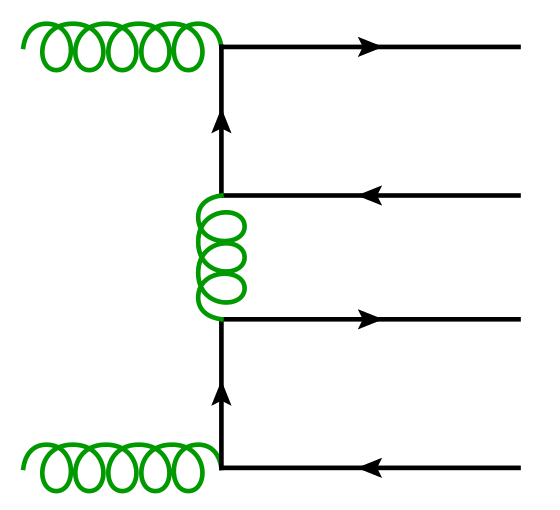
\includegraphics[width=\textwidth]{figures/production-qcd.png}
    }
    \only<3>{%
      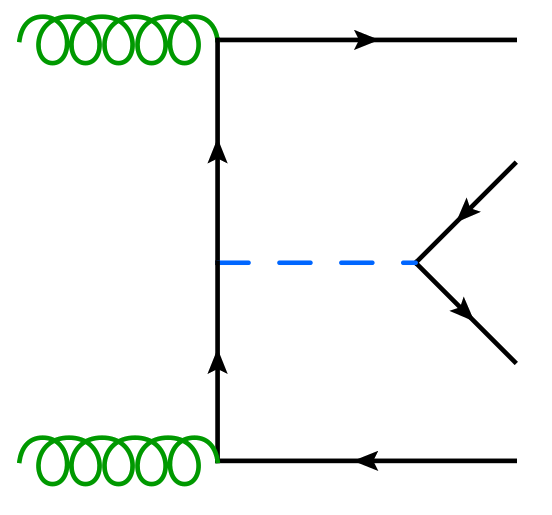
\includegraphics[width=\textwidth]{figures/production-higgs.png}
    }
    \only<4>{%
      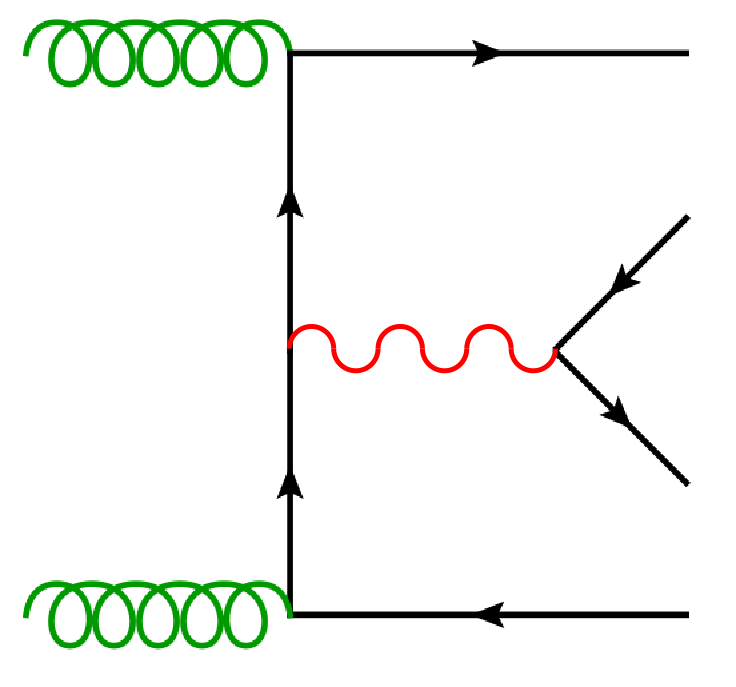
\includegraphics[width=\textwidth]{figures/production-ew.png}
    }
    \only<5>{%
      Standard Model cross-section at $\sqrt{s}=13\mathrm{TeV}$:
      \begin{center}
        \Huge{12.32\fb}
      \end{center}
    }
    \only<6->{%
      Standard Model cross-section at $\sqrt{s}=13\mathrm{TeV}$:
      \vspace{-.15in}
      \begin{center}
        \Large{12.32\fb}
      \end{center}
      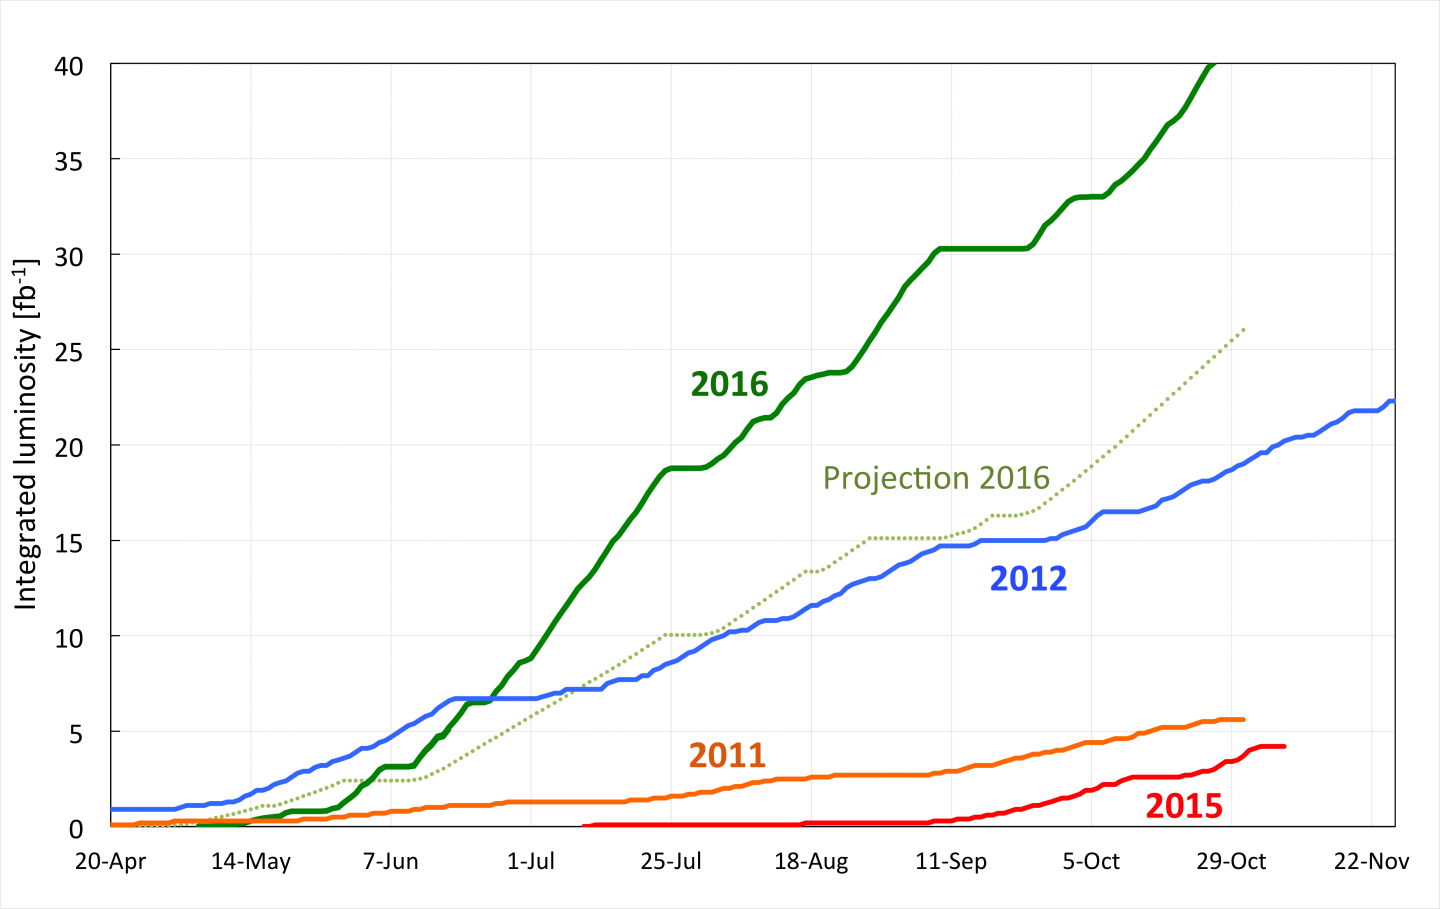
\includegraphics[width=\textwidth]{figures/lhc-luminosity-2016.png}
      % IMGSRC: https://home.cern/cern-people/updates/2016/12/lhc-report-far-beyond-expectations
      \vspace{-.15in}
      \begin{equation*}
        \mathrm{\#\ Signal\ Events}=12.32\fb * 40\invfb \approx 493
      \end{equation*}
    }
  \end{minipage}
\end{frame}

\begin{frame}{Decay Channels}
  \begin{minipage}[c][\textheight]{0.45\textwidth}
    \begin{itemize}
        %TODO: Check the limits on non-bW decays
      \item<1-> All* tops will immediately decay to a b-quark and a W-boson
      \item<2-> The W-boson will immediately decay either
        \begin{itemize}
          \item<2,4-> \textbf{Leptonically}
          \item<3-> \textbf{Hadronically}
        \end{itemize}
      \item<4-> The b-quark will form some b hadron, travel some macroscopic distance, and then hadronize into a jet.
    \end{itemize}
  \end{minipage}
  \begin{minipage}[c][\textheight]{0.54\textwidth}
    \centering
    \only<1>{%
      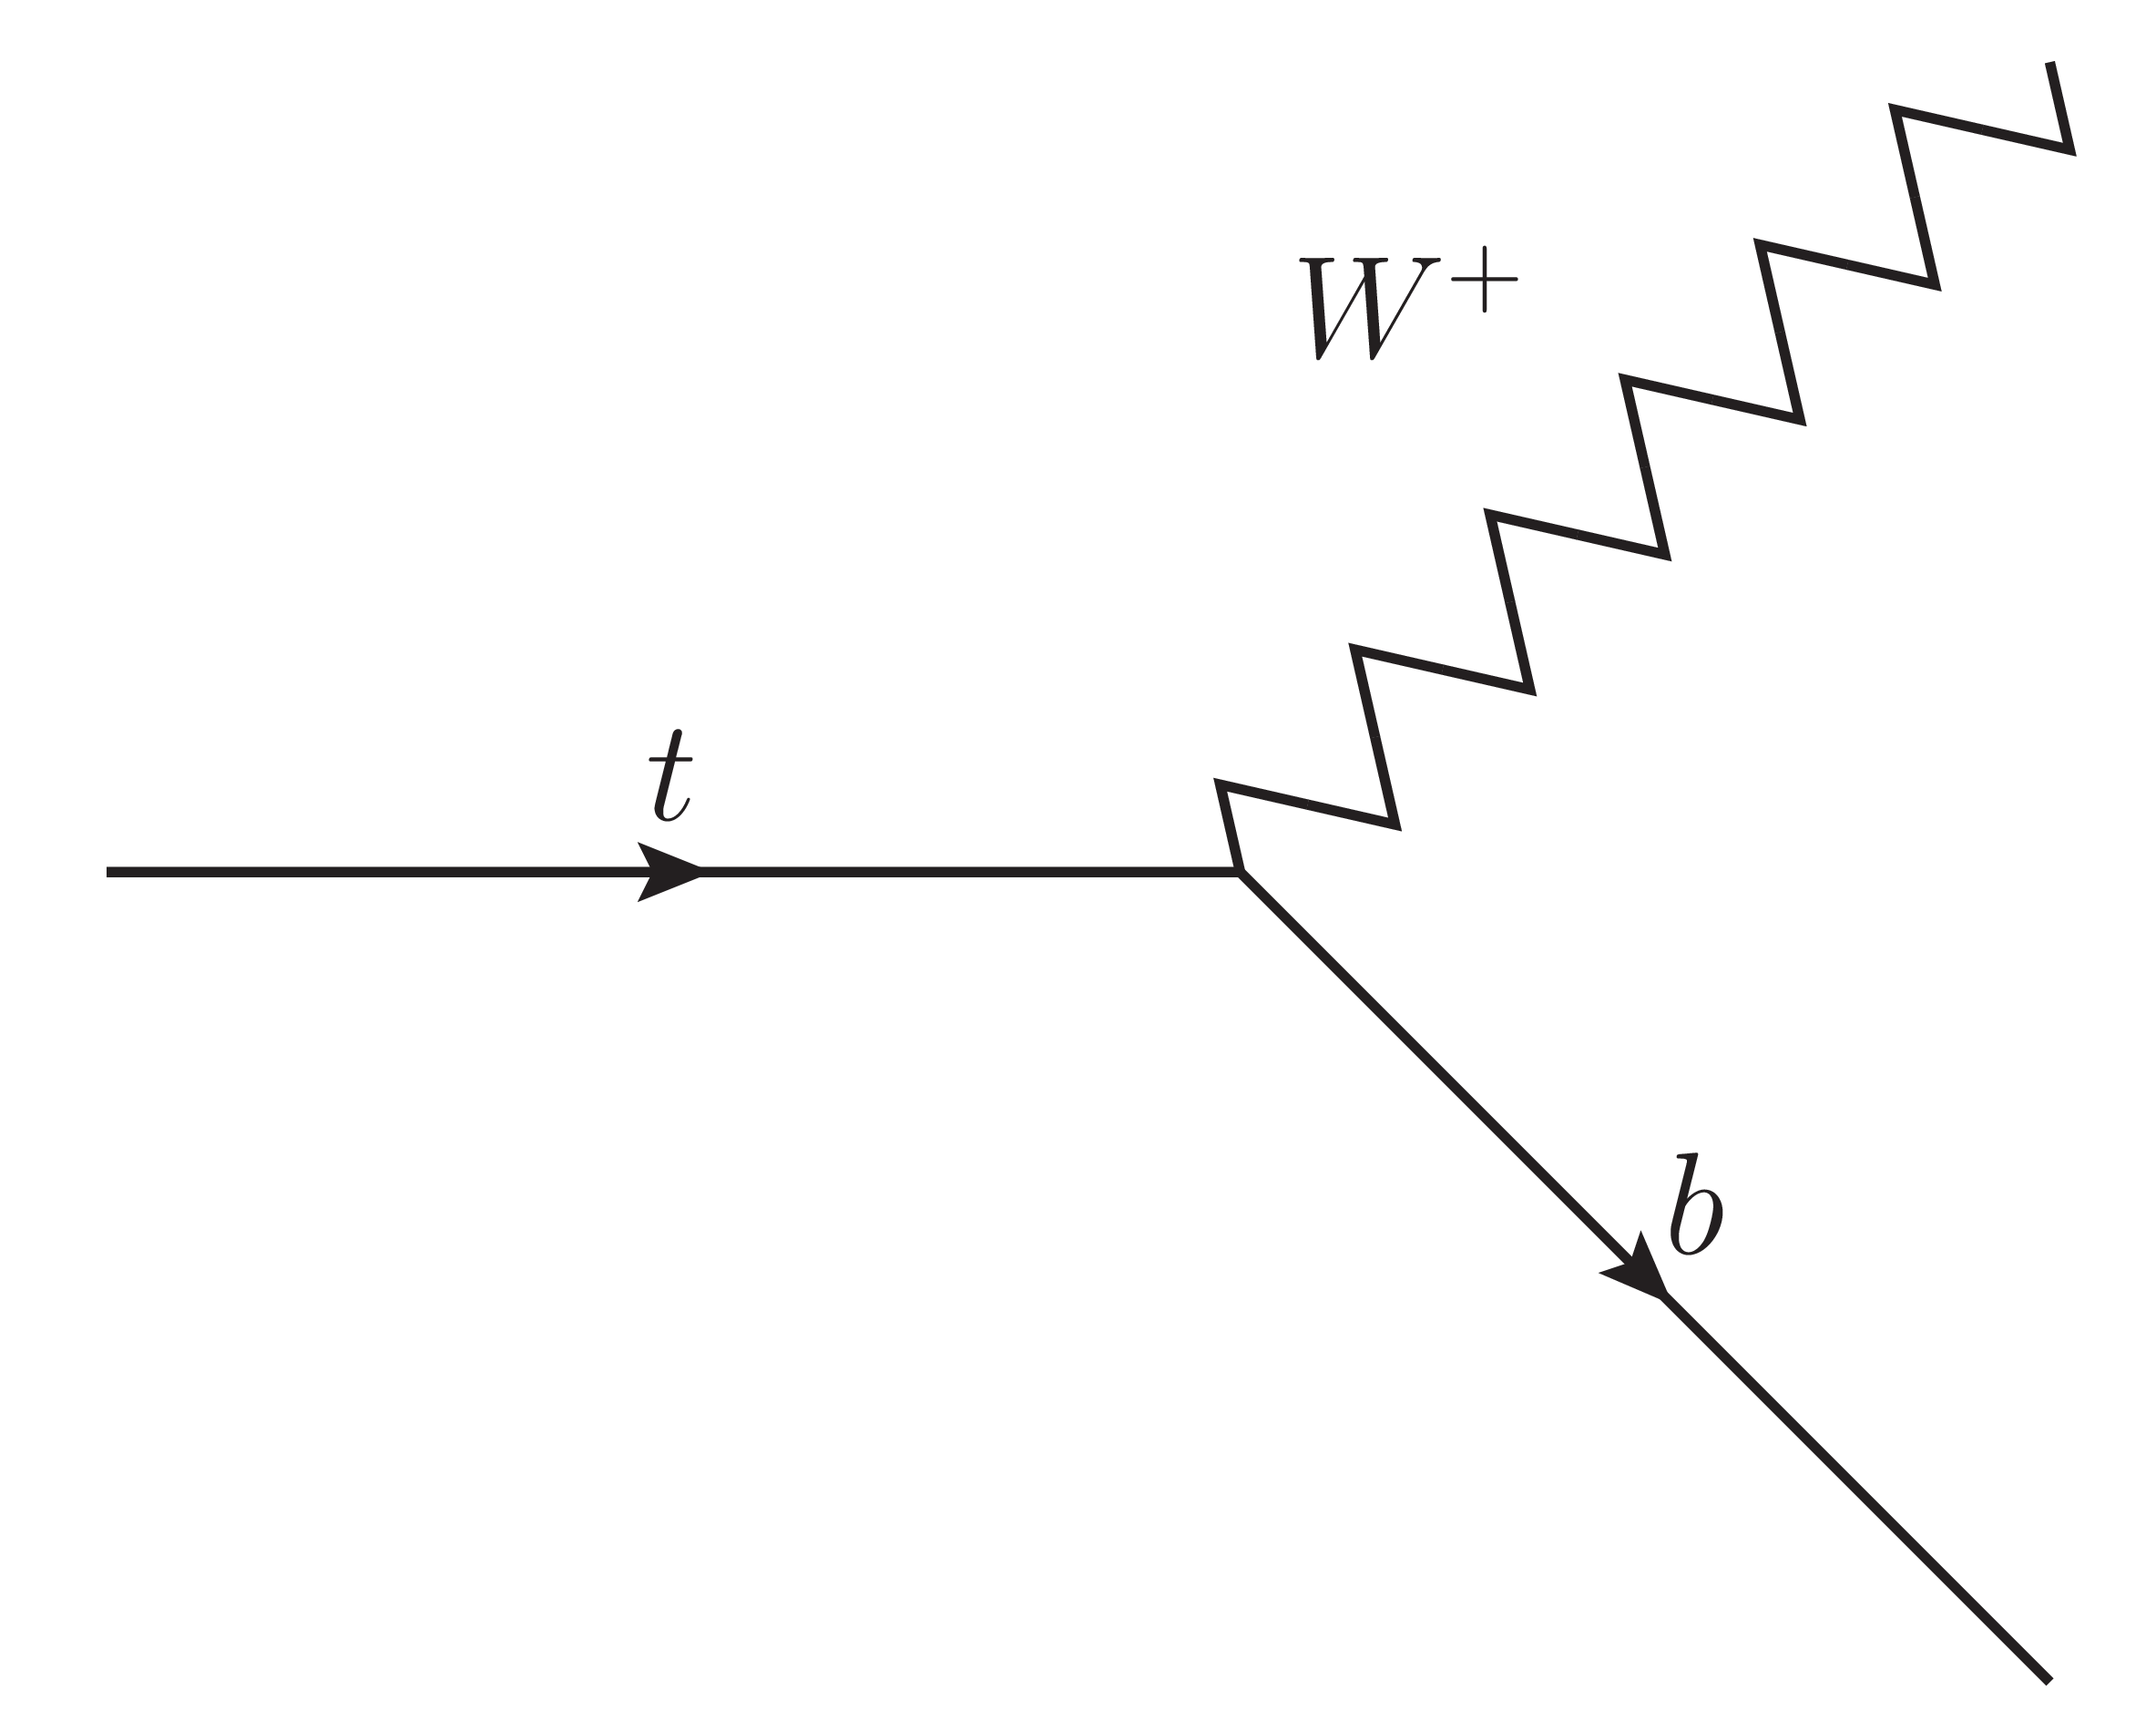
\includegraphics[width=\textwidth]{figures/feynman-diagrams/T->b,W.png}
    }
    \only<2>{%
      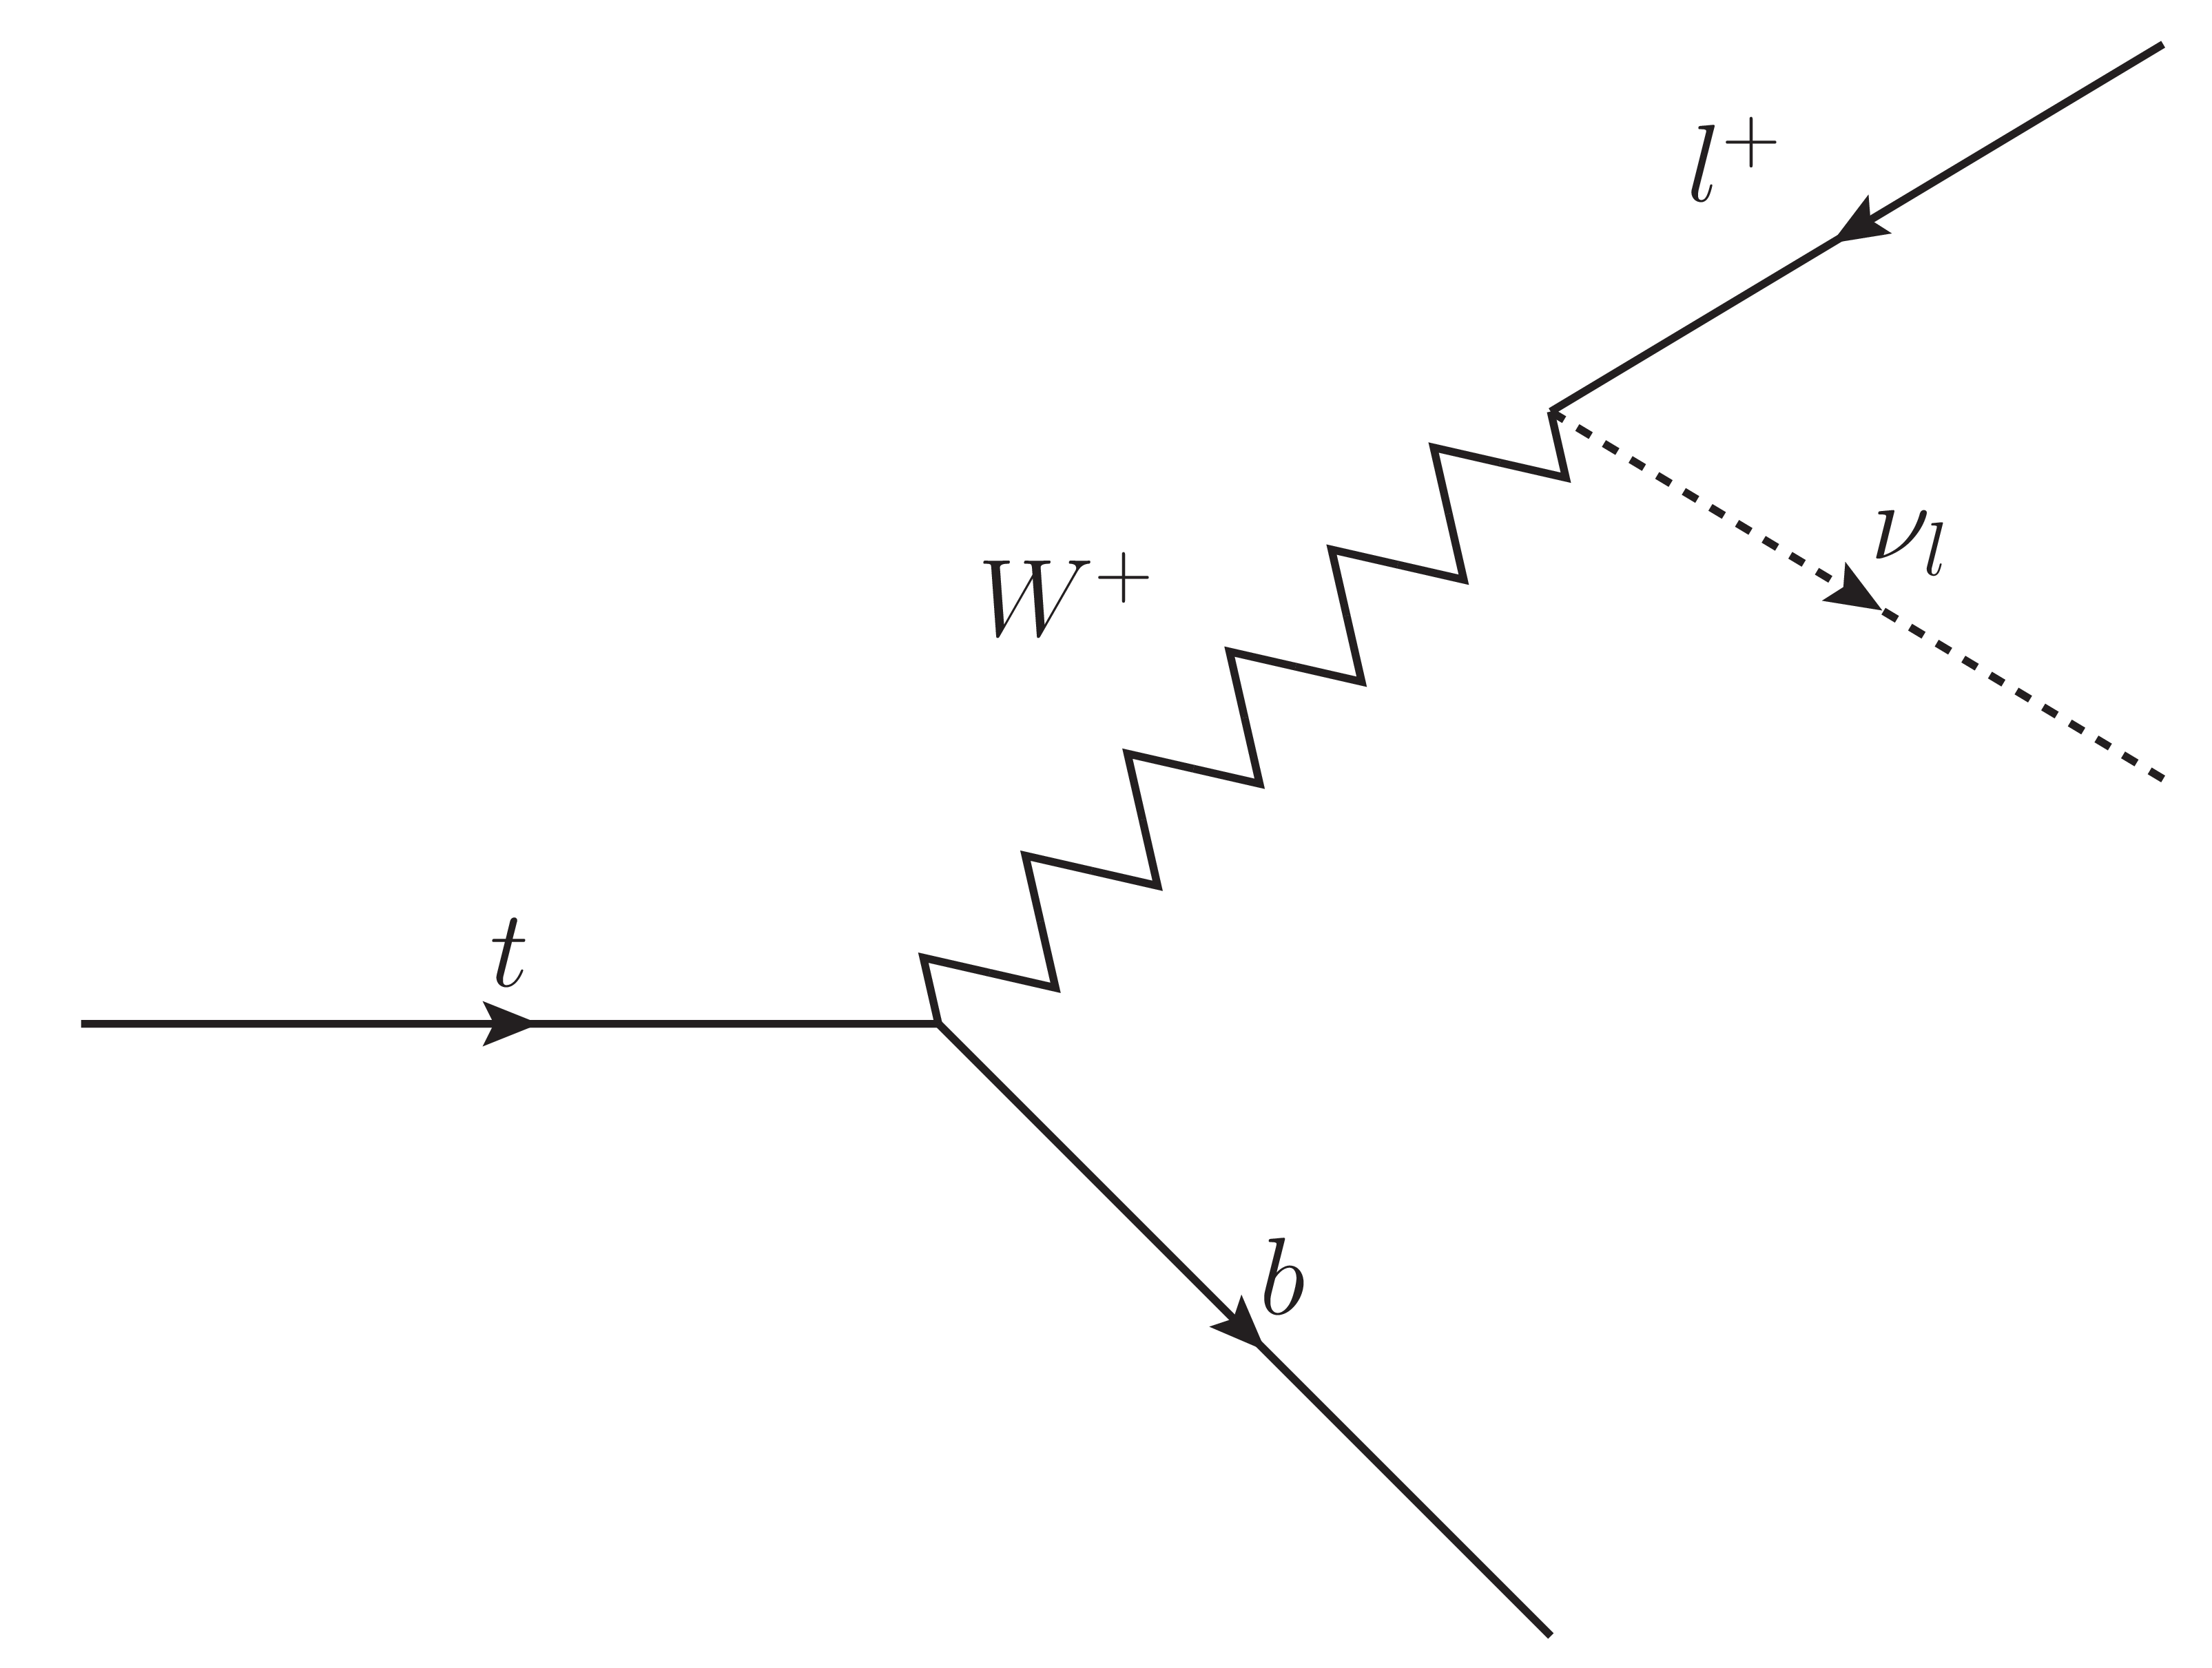
\includegraphics[width=\textwidth]{figures/feynman-diagrams/T->b,(W->ln).png}
    }
    \only<3>{%
      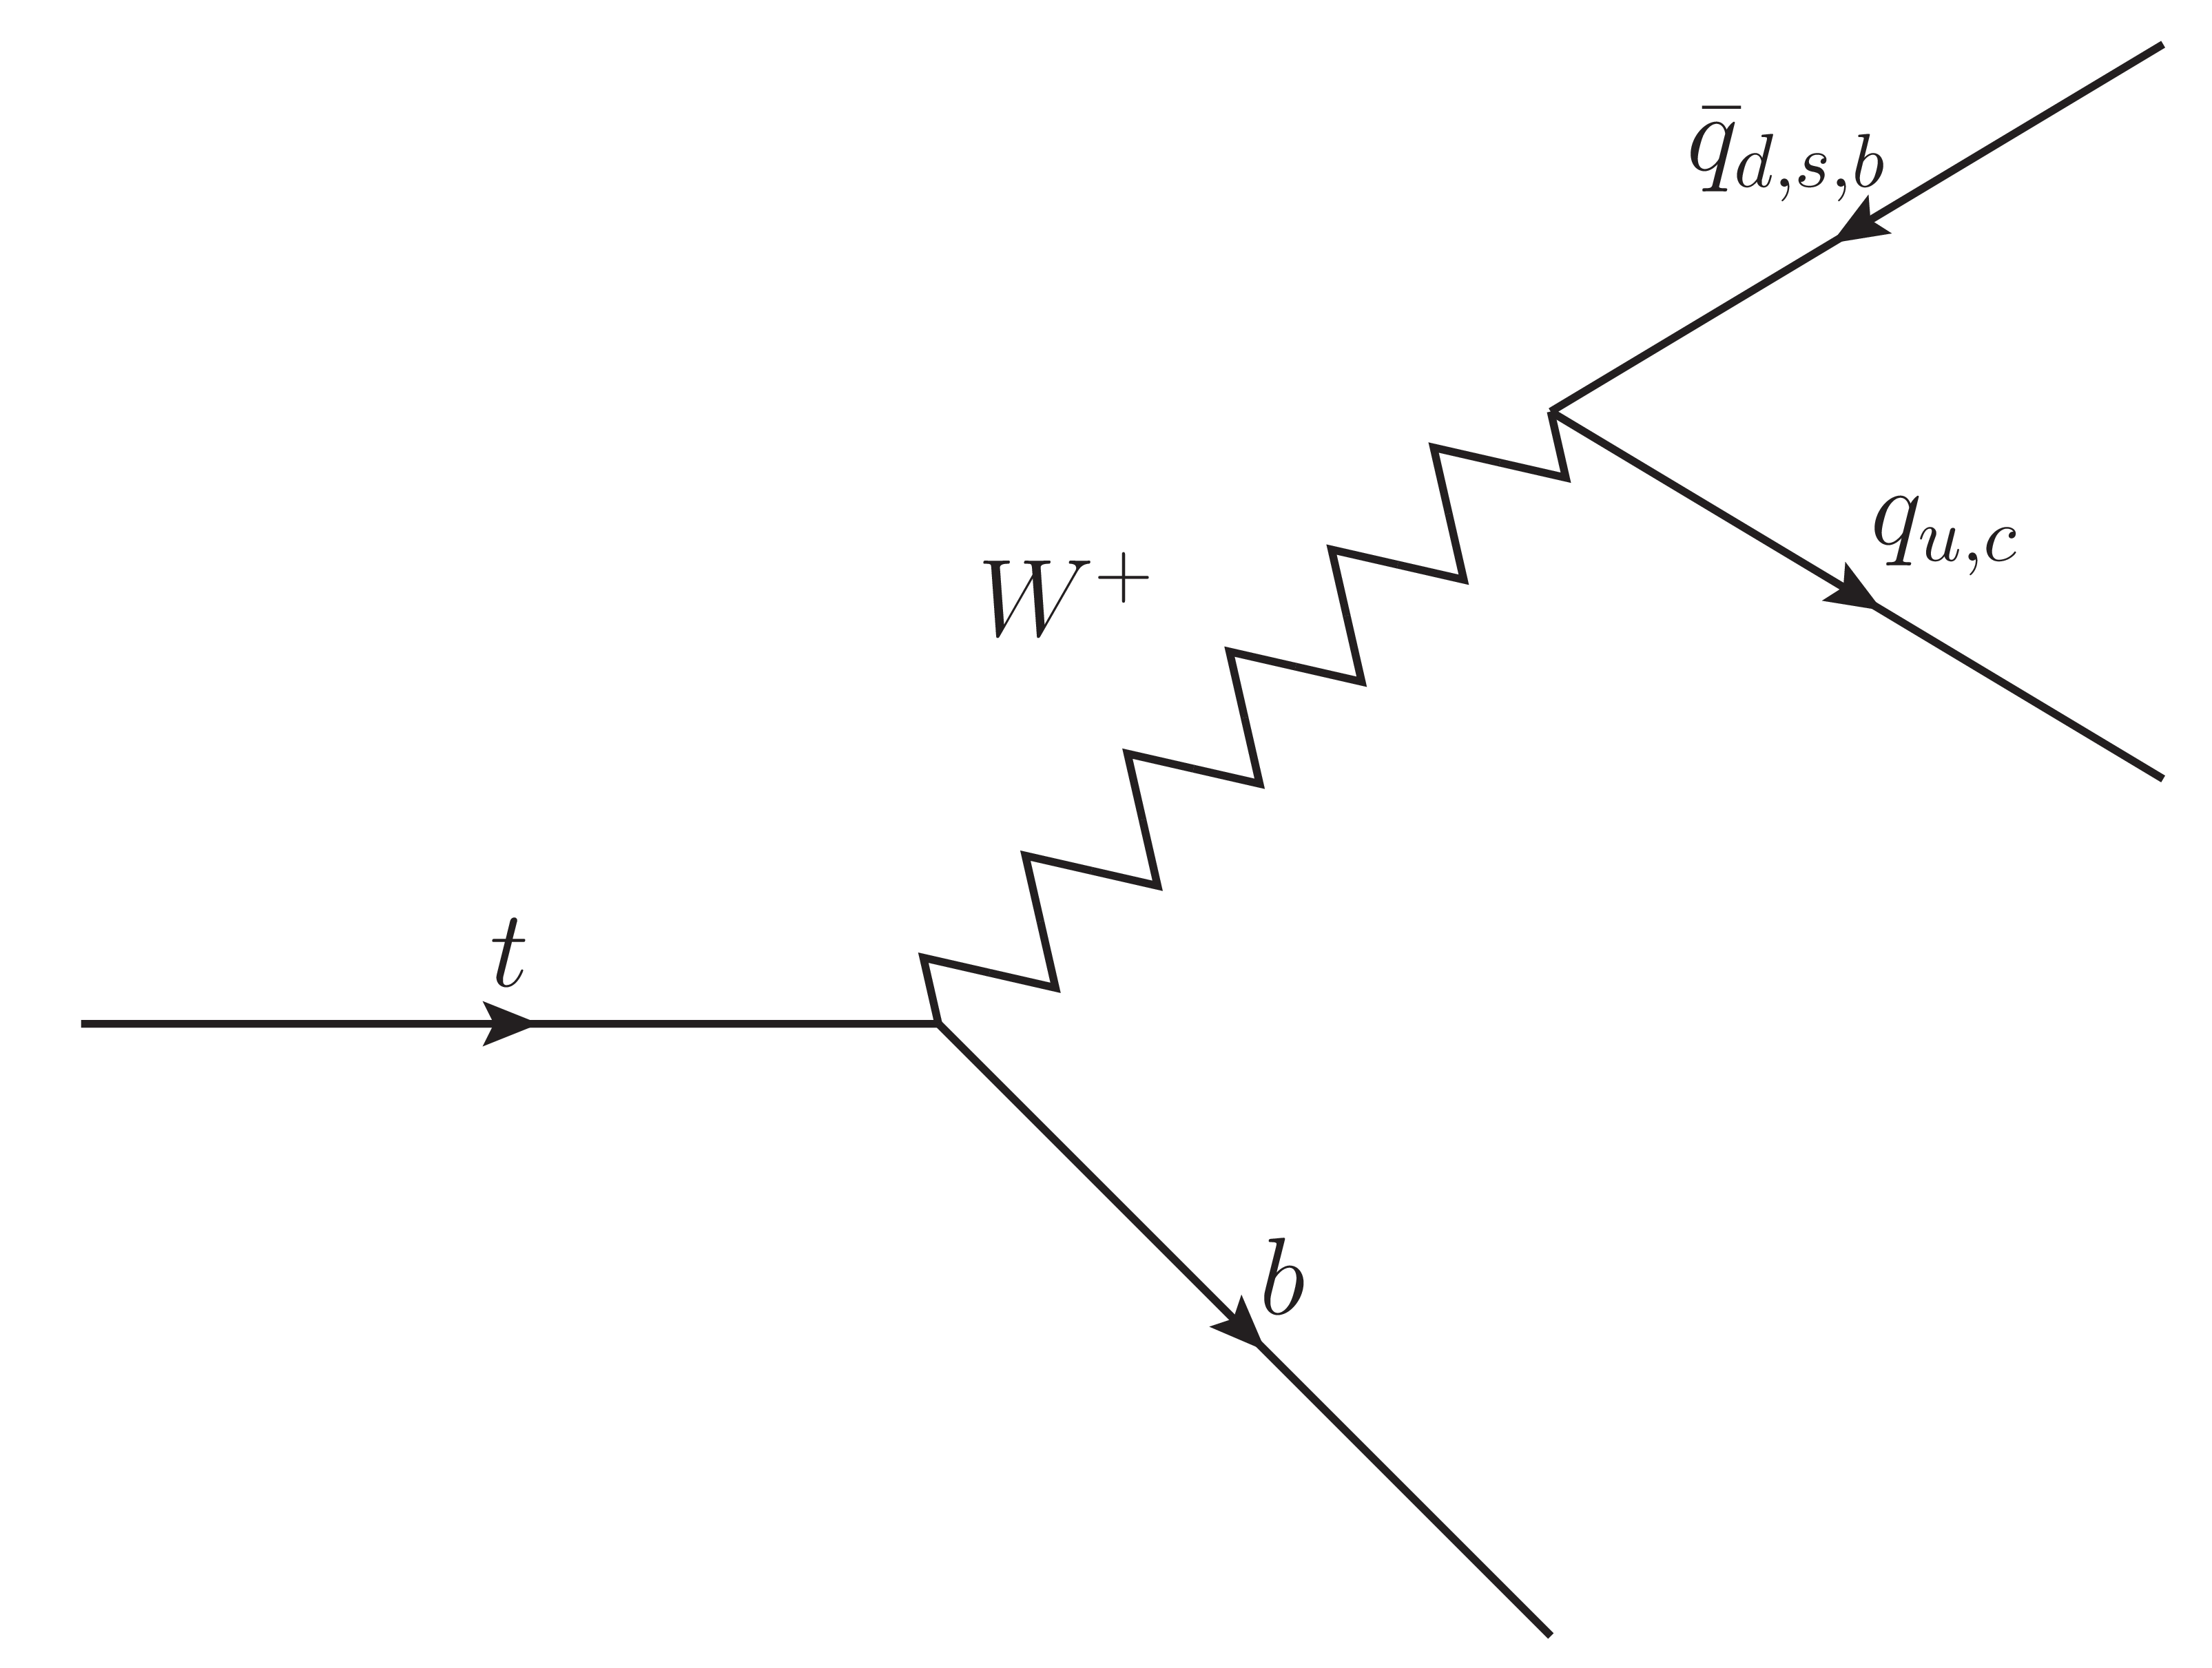
\includegraphics[width=\textwidth]{figures/feynman-diagrams/T->b,(W->qq).png}
    }
    \only<4>{%
      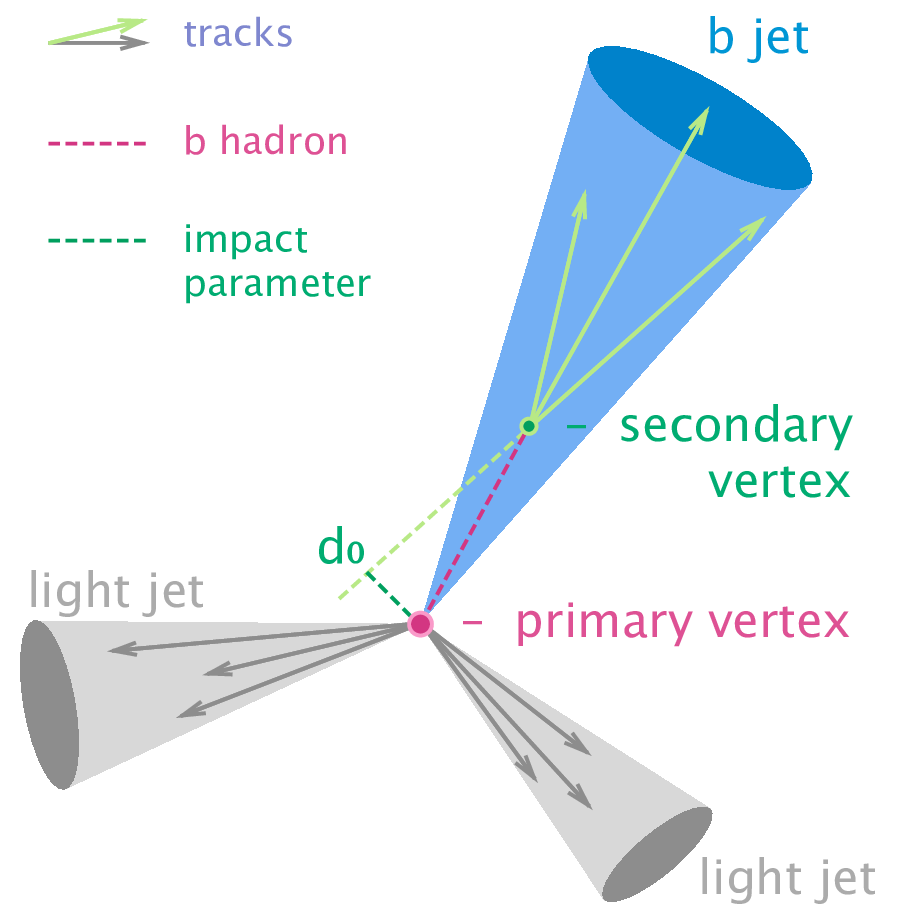
\includegraphics[width=0.90\textwidth]{figures/b-tagging.png}
    }
  \end{minipage}
\end{frame}


\begin{frame}{Decay Channels}
  The Decay channels are enumerated based on the types of W-decays
\begin{table}[]
  \tiny
  \begin{tabular}{@{}llccrrc@{}}
    \textbf{Name}               & \textbf{Leptons}           & \textbf{B-Jets} & \textbf{LF-Jets} & \textbf{BR}     & \textbf{BR ($\mu$ and $e$ only)} & \textbf{Events @ 40\invfb}    \\ \midrule
  Hadronic                    &                            & 4               & 8                & 20\%            & 20\%                             & 99                               \\ \midrule
  Single Lepton               & $\ell^\pm$                 & 4               & 6                & 40\%            & 26.6\%                           & 131                              \\ \midrule
  Same-Sign (SS) Dilepton     & $\ell^\pm \ell^\pm$        & 4               & 4                & 9.7\%           & 4.3\%                            & 21                               \\ \midrule
  Opposite-Sign (OS) Dilepton & $\ell^\pm \ell^\mp$        & 4               & 4                & 19.3\%          & 8.6\%                            & 42                               \\ \midrule
  Trilepton                   & $\ell^\pm\ell^\pm\ell^\mp$ & 4               & 2                & 9.8\%           & 2.9\%                            & 14                               \\ \midrule
  Leptonic                    & $\ell^+\ell^+\ell^-\ell^-$ & 4               & 2                & 1.2\%           & 0.24\%                           & 1                                \\ \bottomrule
  \end{tabular}
\end{table}
\vfill
\footnotesize{$\ell \in \left(e,\mu,\tau\right)$}
\end{frame}

\section{Previous Measurements}
\begin{frame}{Previous CMS Measurements @ 13TeV}
\begin{table}[]
  \begin{tabular}{@{}lcr@{}}
  \textbf{Analysis}           & \textbf{Channel}            & \textbf{Limit}  \\ \midrule
  CMS-TOP-16-016              & Single Lepton, OS Dilepton  & 94\fb          \\ \midrule
  CMS-SUS-15-008              & SS Dilepton                 & 119\fb         \\ \bottomrule
  \textbf{Combined}           &                             & 69\fb          \\
  \end{tabular}
\end{table}
\end{frame}

\section{Strategy}
\begin{frame}{Strategy}
\end{frame}

\section{Progress \& Status}
\begin{frame}{Progress \& Status}
\end{frame}

\section{Conclusions}
\begin{frame}{Conclusions}
\end{frame}

\end{document}
